\chapter{\xlabel{fcfstime}FCFs by Time of Night}
\label{app:fcfstime}

\cref{Figure}{fig:FCFsTimeOfNight}{} shows the Beam (Peak) FCFs at
450 and 850\,$\mu$m as a function of UT time for observations of the
primary calibrator, Uranus along with secondary calibrators CRL~2688, and CRL~618.
The Peak FCF is larger in the evening and morning primarily because thermal
deformations of the dish dilute the flux from the main beam into the secondary
(error) component (see Mairs et al. 2021~\cite{mairs21}). There is no significant
change to the Arcsecond FCFs in the early evening or late morning.

\begin{figure}
\begin{center}
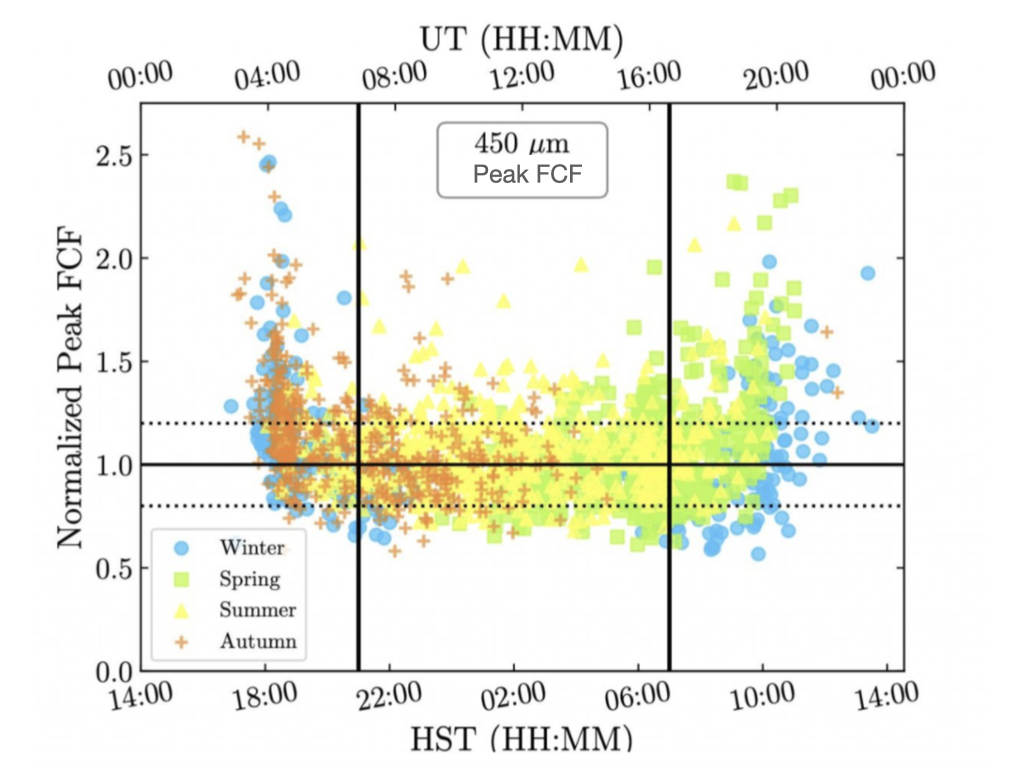
\includegraphics[width=0.47\linewidth]{sc21-FCFsTimeOfNight-450} \hspace{0.02\linewidth}
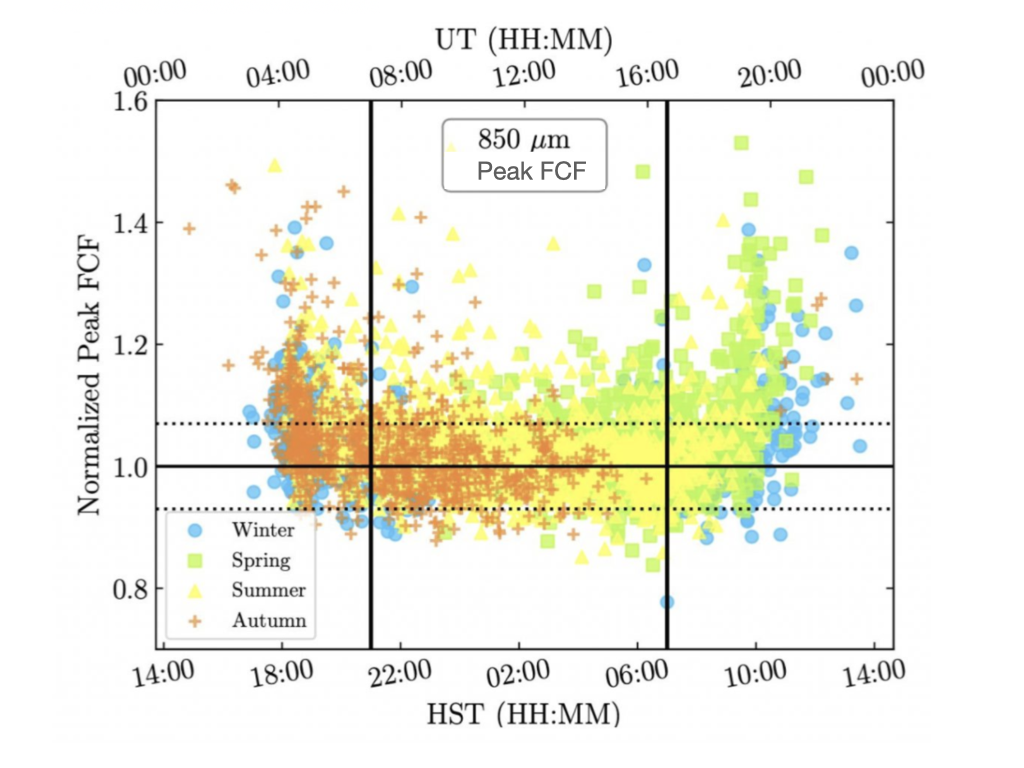
\includegraphics[width=0.47\linewidth]{sc21-FCFsTimeOfNight-850}
\caption[FCFs Time of Night]{The Normalized Peak FCFs at 450 (left) and 850\,$\mu$m (right)
as a function of observation time. All FCFs are derived using the primary calibrator Uranus and
secondary calibrator CRL~2688. The vertical lines mark the beginning and end of the “stable” observation
period from 07:00–-17:00 (UTC). The horizontal (dotted) lines show the FCF uncertainties derived for the
stable observation period around a value of 1.0 (horizontal, solid line).
Data are coloured according to season. \label{fig:FCFsTimeOfNight}}
\end{center}
\end{figure}

\cref{Figure}{fig:FCFsTimeOfNightFits}{} show the Peak FCF trends in detail for evening and morning
observations of Uranus and CRL~2688. The data are bootstrap-fitted with linear functions and ``rs''
indicates the Spearman rank correlation of the fit.

\begin{figure}
\begin{center}
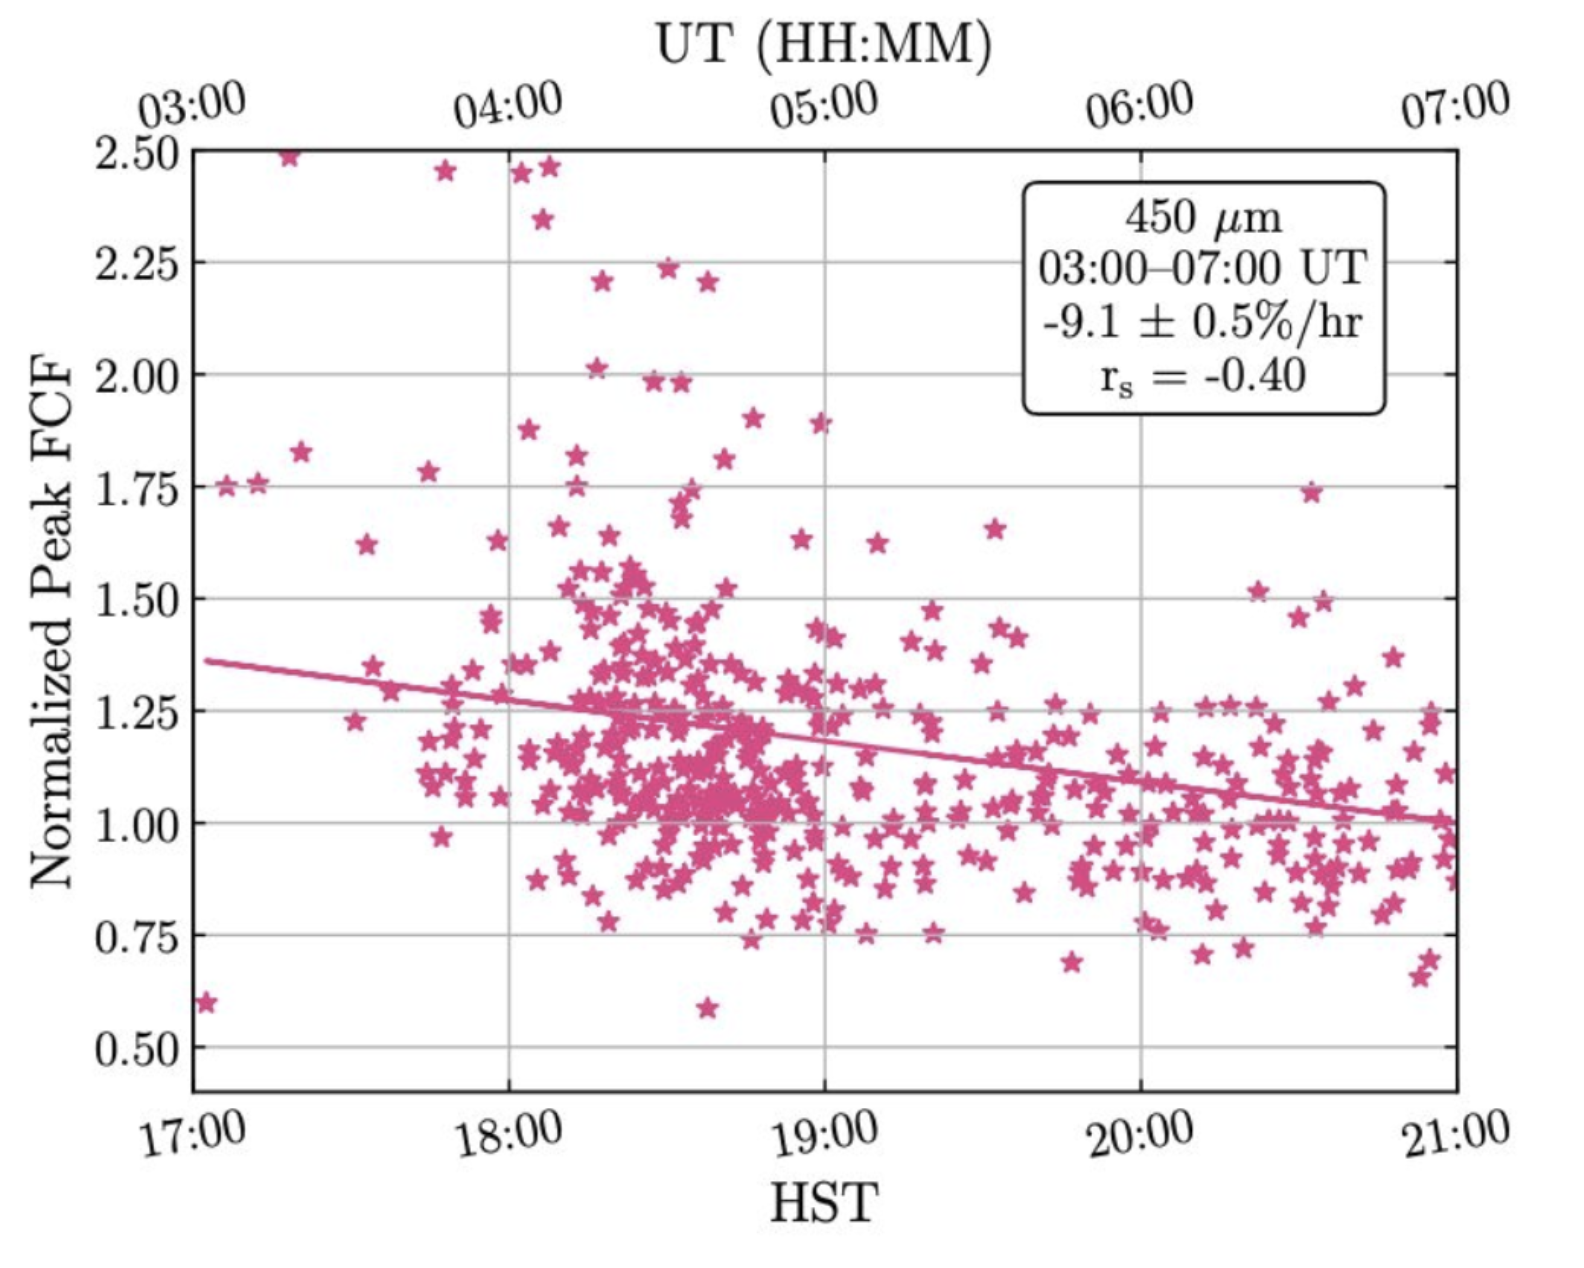
\includegraphics[width=0.47\linewidth]{sc21-FCFsTimeOfNightFitsE-450} \hspace{0.02\linewidth}
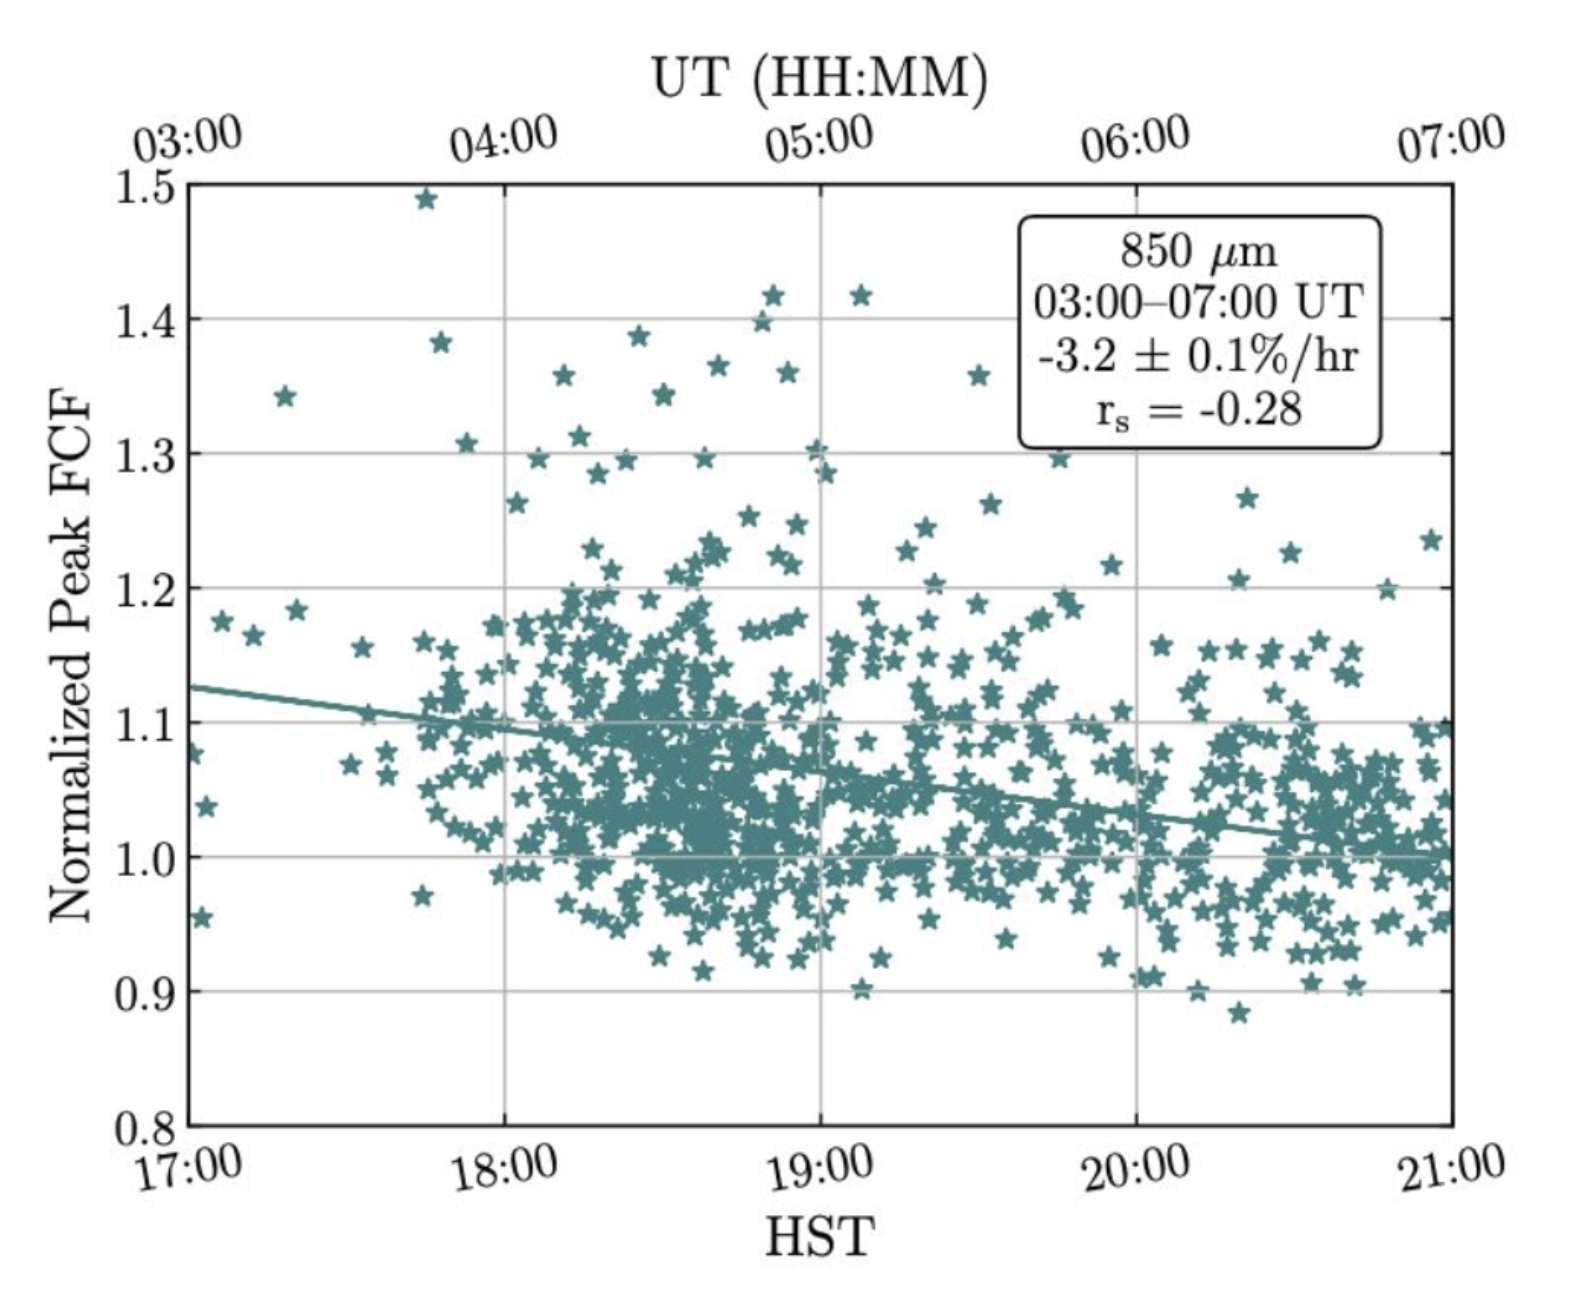
\includegraphics[width=0.47\linewidth]{sc21-FCFsTimeOfNightFitsE-850}\\
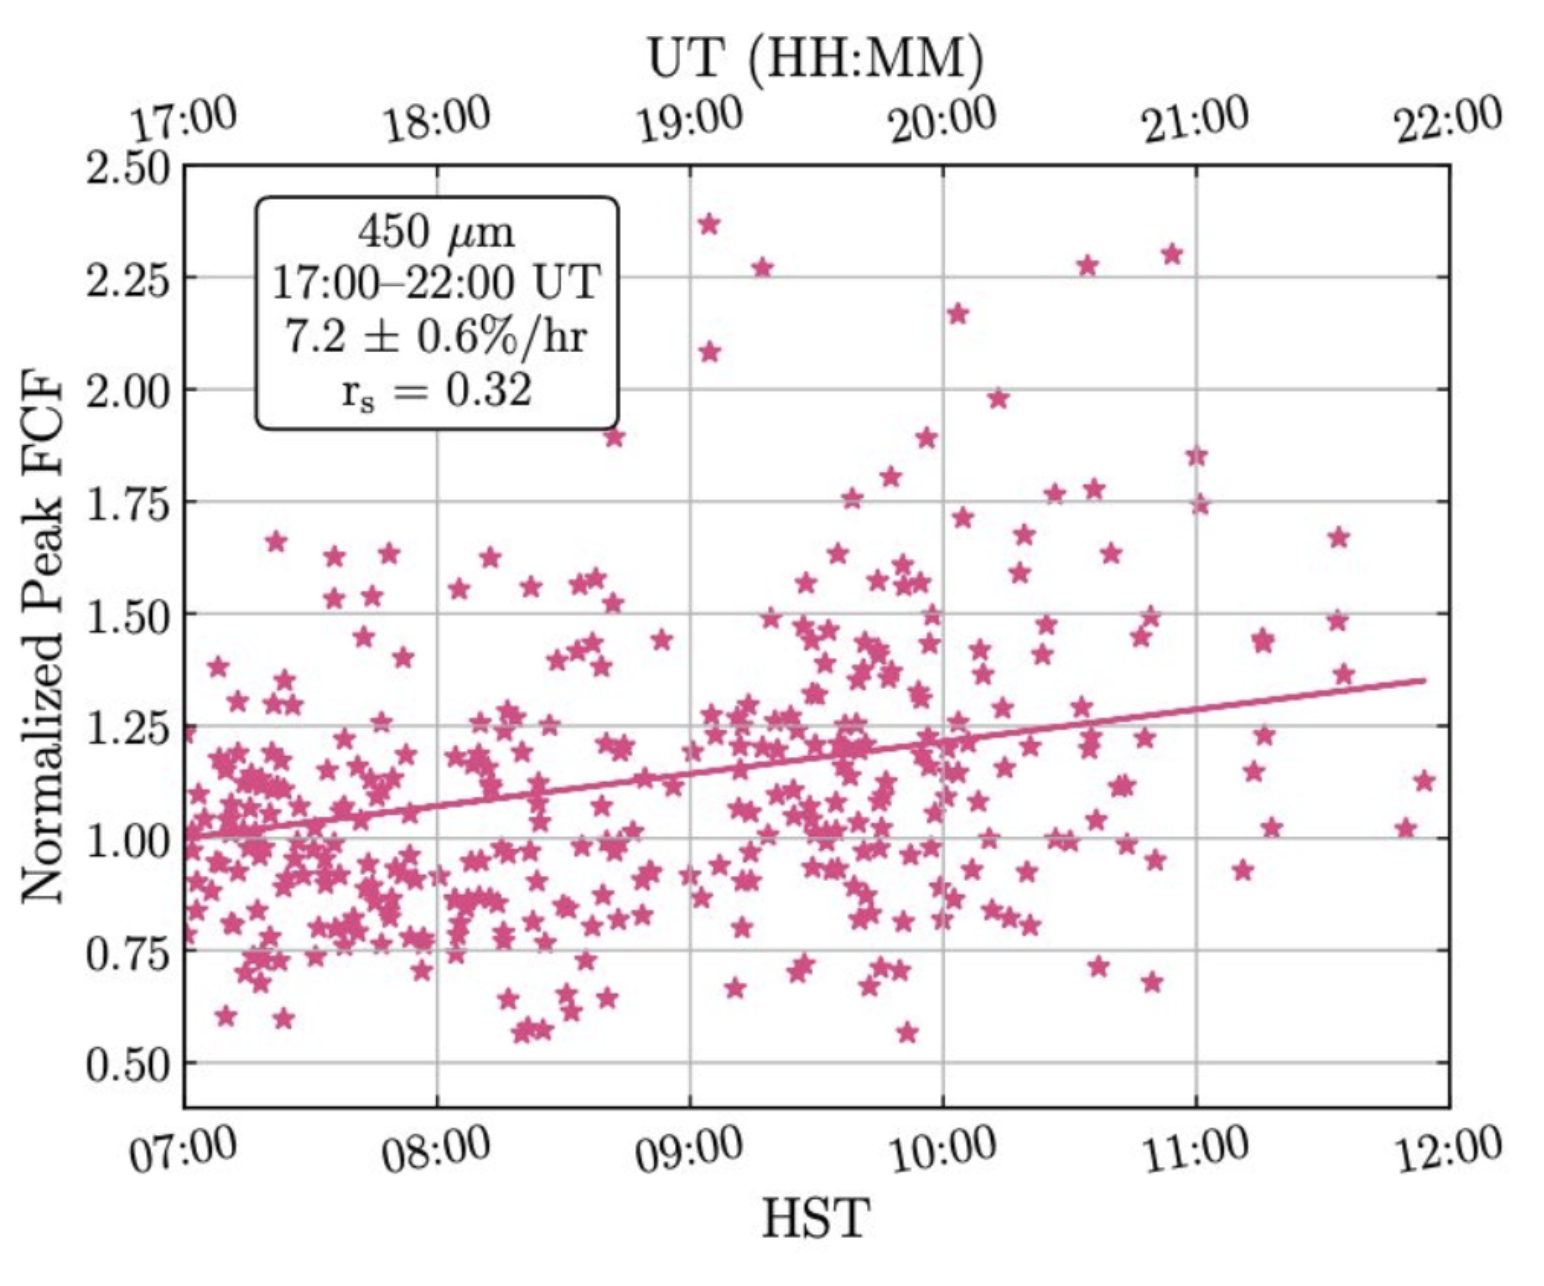
\includegraphics[width=0.47\linewidth]{sc21-FCFsTimeOfNightFitsM-450} \hspace{0.02\linewidth}
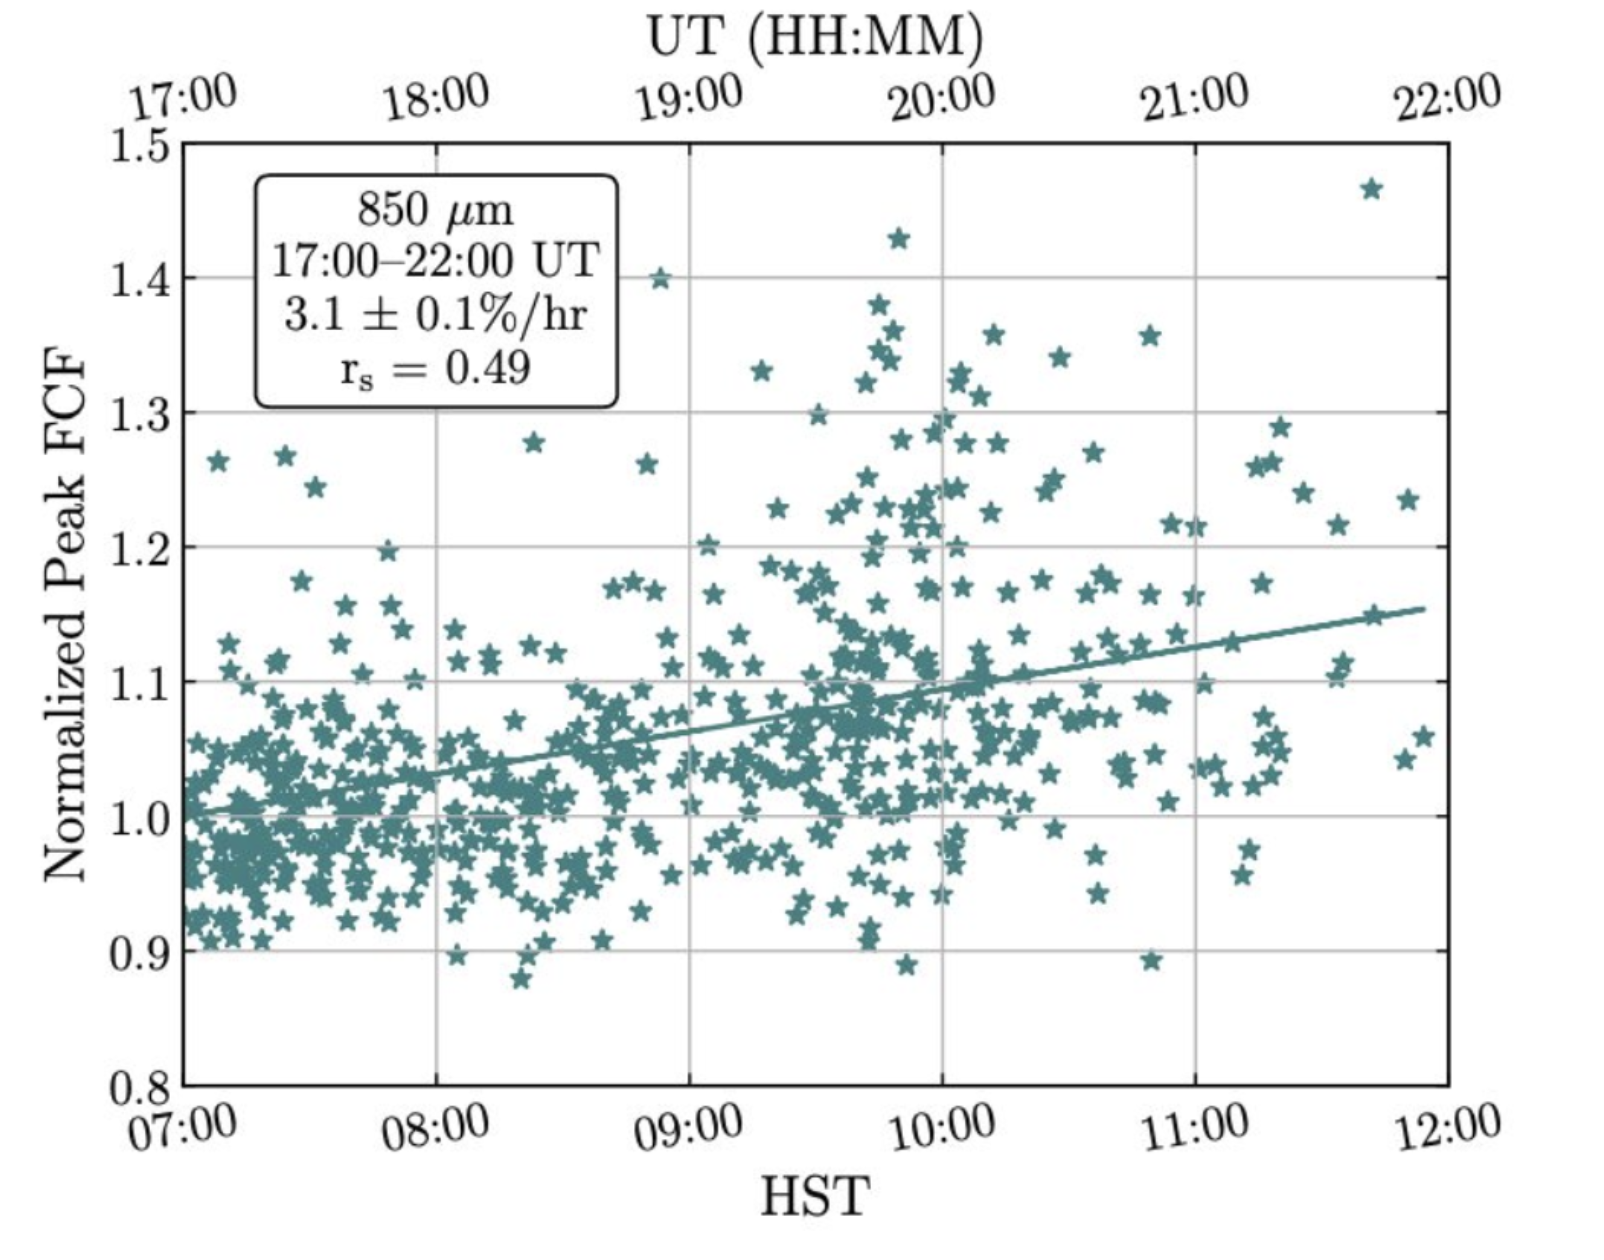
\includegraphics[width=0.47\linewidth]{sc21-FCFsTimeOfNightFitsM-850}
\caption[FCFs Time of Night Fits]{Linear fits to the Peak FCFs at 450\,$\mu$m (left) and 850\,$\mu$m (right)
 during the evening (top) and morning (bottom) when dish distortions caused by thermal gradients affect the
 beam shape. The distributions during the stable part of the night (07:00--17:00 UTC) show no significant
 slope and therefore require no corrections to the default FCFs shown in
 \cref{Appendix}{app:fcfs}{FCFs by reduction date}. \label{fig:FCFsTimeOfNightFits}}
\end{center}
\end{figure}


The Peak FCFS DECREASE in the evening as the ambient temperature cools and the dish settles, while
the Peak FCFS INCREASE in the morning as the ambient temperature warms and the dish becomes
unstable to thermal gradients. \cref{Table}{tab:FCFsTimeOfNight}{below} summarises the rate of change.
As of Starlink Release 2021A, \oracdr\ \textbf{does not} apply these corrections by default. If
you wish to apply these corrections, the FCFs must be modified manually (see
\cref{Section}{subsec:ApplyingFCF}{Manually applying the FCF}).


\begin{table}[h!]
\begin{center}
\begin{tabular}{|c|c|c|}
 \hline
 \multicolumn{1}{|c|}{Wavelength} &
 \multicolumn{1}{c|}{Time Range (UTC)} &
 \multicolumn{1}{c|}{Peak FCF Correction (\% hr$^{-1}$)}
 \\ \hline
$450\,\mu$m & 03:00--07:00 & $9.1\pm0.5$ \\
$450\,\mu$m & 17:00--22:00 & $7.2\pm0.6$ \\
\hline
$850\,\mu$m & 03:00--07:00 & $3.2\pm0.1$ \\
$850\,\mu$m & 17:00--22:00 & $3.1\pm0.1$ \\ \hline
\end{tabular}
\end{center}
\label{tab:FCFsTimeOfNight}
\end{table}

